
\begin{figure*}[ht!]
\centering
\begin{tabularx}{0.92\textwidth}{c c c}
%\begin{tabularx}{}
%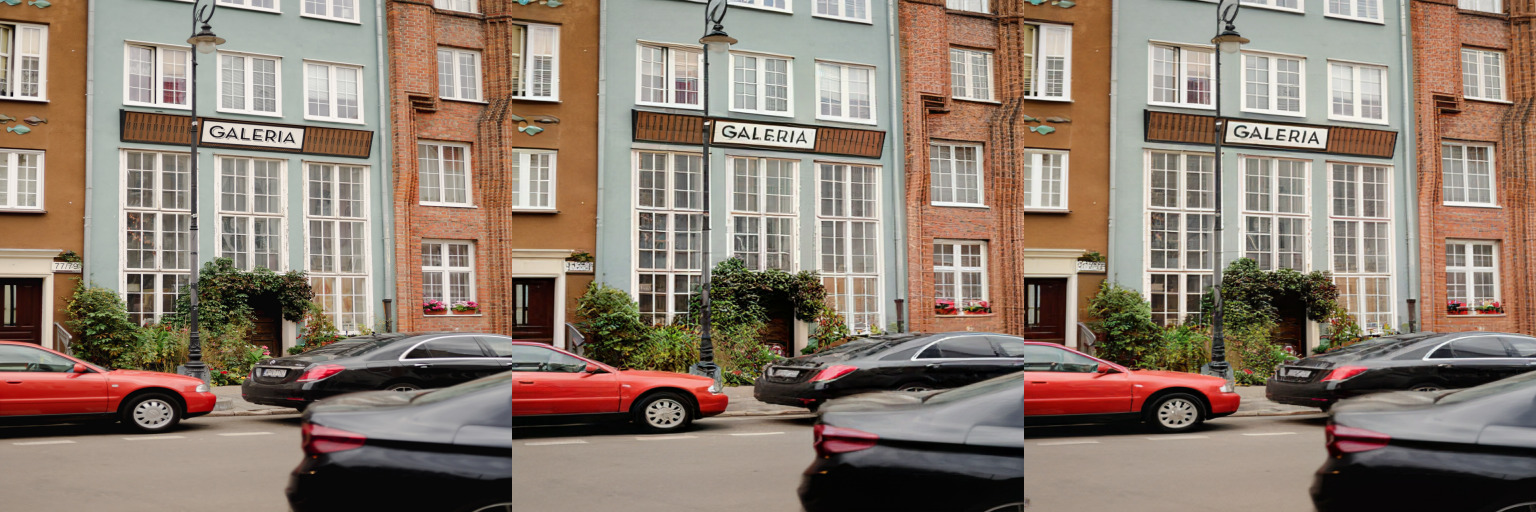
\includegraphics[width=0.90\textwidth]{figs/fine_tune_decoder/free6_grid}
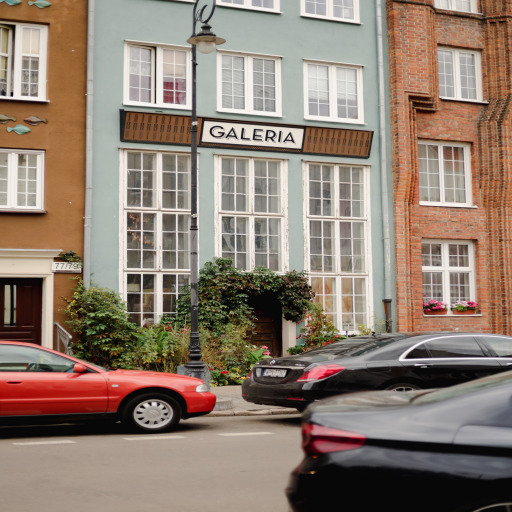
\includegraphics[width=0.30\textwidth]{figs/fine_tune_decoder/free6_ori} &
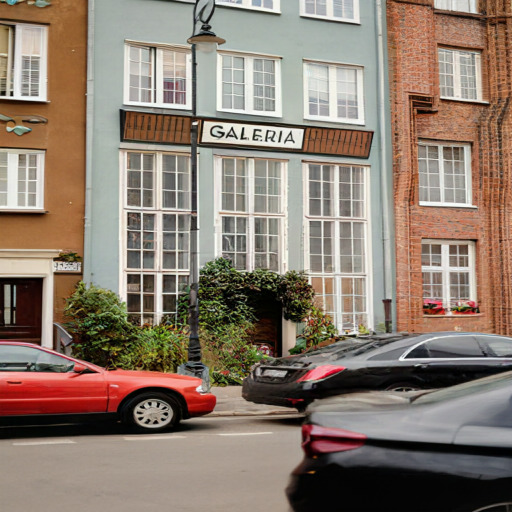
\includegraphics[width=0.30\textwidth]{figs/fine_tune_decoder/free6_reconstruced} &
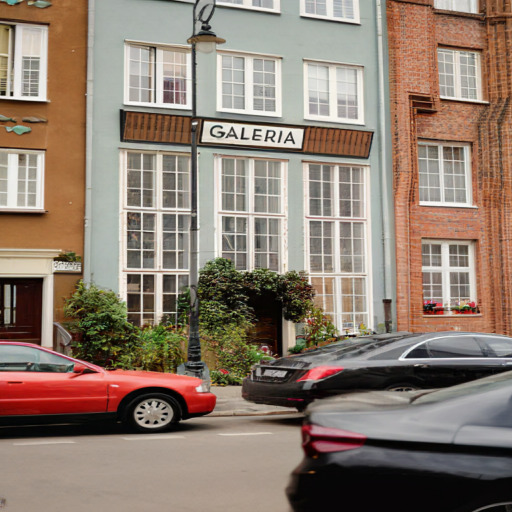
\includegraphics[width=0.30\textwidth]{figs/fine_tune_decoder/free6_ft_reconstruced}

\\
Input Image &
VQGAN Reconstruction &
Finetuned Decoder 

\end{tabularx}
\caption{\small Visual example of the improvement from the fine-tuned decoder (\cref{sec:dec_finetune}). Please zoom in by at least 200\% to see the difference between the VQGAN reconstruction and the reconstruction with a finetuned decoder. We can see especially that fine details such as the house number (bottom left), the storefront sign (middle) and the bars on the windows (right) are better preserved in the finetuned decoder.}
\label{fig:finetune_decoder}
\end{figure*}
